\documentclass[tikz,border=5pt]{standalone}
\usepackage{tikz}

\begin{document}

% Logo: Multiple paths converging into one clean line
% Suggests: chaos → order, multi-author → unified output
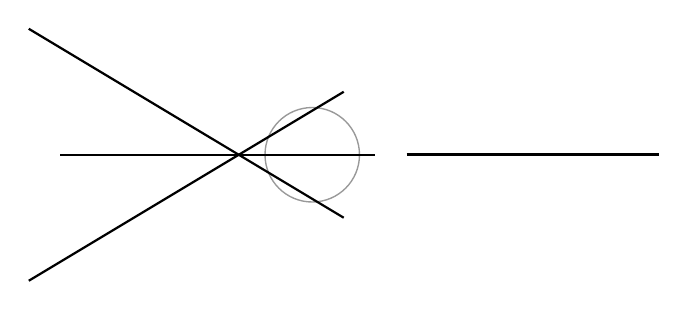
\begin{tikzpicture}[scale=4]
  % Three incoming lines (chaotic, misaligned)
  \draw[line width=0.8pt] (-0.8, 0.4) -- (0.2, -0.2);
  \draw[line width=0.8pt] (-0.7, 0) -- (0.3, 0);
  \draw[line width=0.8pt] (-0.8, -0.4) -- (0.2, 0.2);
  
  % One clean outgoing line (aligned, structured)
  \draw[line width=1.2pt] (0.4, 0) -- (1.2, 0);
  
  % Convergence point - subtle circle
  \draw[line width=0.5pt, opacity=0.4] (0.1, 0) circle (0.15);
  
\end{tikzpicture}

\end{document}
